\chapter{Fundamentação Teórica}
    Este capitulo busca contextualizar os principais conceitos abordados no presente trabalho, tais como os materiais
    utilizados como base e também a tecnologia adotada no desenvolvimento do projeto. E ao final, serão elencados alguns
    trabalhos correlatos.

    \section{ENEF}
        Buscando consolidar a cidadania da população brasileira foi criada a Estratégia Nacional de Educação Financeira
        (ENEF), que possui como áreas de estudo, as seguintes: direitos, deveres, investimento, previdência, poupança,
        crédito, seguros, consumo e planejamento. A estratégia tem o público que inicia desde a escola até a fase adulta,
        de maneira a proporcionar atividades condizentes com cada faixa etária, abordando todas as áreas de estudo.
        Todos os processos e planos de ações adotados pela ENEF são baseados em seu plano diretor, que detalha a
        relevância destes conhecimentos para que se tenha uma população mais consciente, este documento também detalha
        sobre quais cenários devem implementadas as ações.

        \subsection{Material Didático}
            Foram disponibilizados pela estratégia um total de 24 livros, onde 18 são destinados ao Ensino Fundamental e
            os outros 6 são para o Ensino Médio. Os livros são divididos em 12 para alunos e 12 para os professores,
            estes materiais têm o objetivo de transmitir os conteúdos propostos pela ENEF para os alunos durante sua
            vida escolar.

            Os livros do se iniciam no primeiro ano do Ensino Fundamental, com conceitos muito simples que vão moldando
            a cidadania das crianças, conceitos como planejamento e organização que são aplicados de forma prática para
            organização da sala de aula e de festas. O material também apresenta a origem de produtos comuns do dia a
            dia como batatas, leite e a bola. A partir do livro 3 começam a ser introduzidos conceitos financeiros
            básicos, sendo realizada uma introdução as contas domésticas, como elas são calculadas conforme o consumo de
            cada equipamento. Após isso tem-se o início da contextualização do dinheiro físico e como ele é feito e
            usado e por fim reciclado.

            No 5º e 6º livro temos uma dinâmica um pouco diferente, sendo a aplicação de alguns jogos no formato
            livro-jogo, que permite ao usuário tomar decisões que podem o levar por diferentes caminhos e finais,
            algumas das possibilidades estão demonstradas na Figura 1. As alternativas são disponibilizadas ao usuário
            ao final da leitura do cenário e podem conter duas ou três possibilidades de caminhos a seguir, conforme
            Figuras 2 e 3.

            Já nas fases finais do Ensino Fundamental são abordados conceitos e instituições que disponibilizam algum
            recurso para a sociedade, pontuando a atribuição de cada organização. São algumas das organizações estudadas
            : Banco, Agência de Viagens, Hotel, dentre outras.

        \begin{figure}
            \centering
            \caption{Esquema com alguns dos caminhos possíveis da primeiro jogo/história.}
            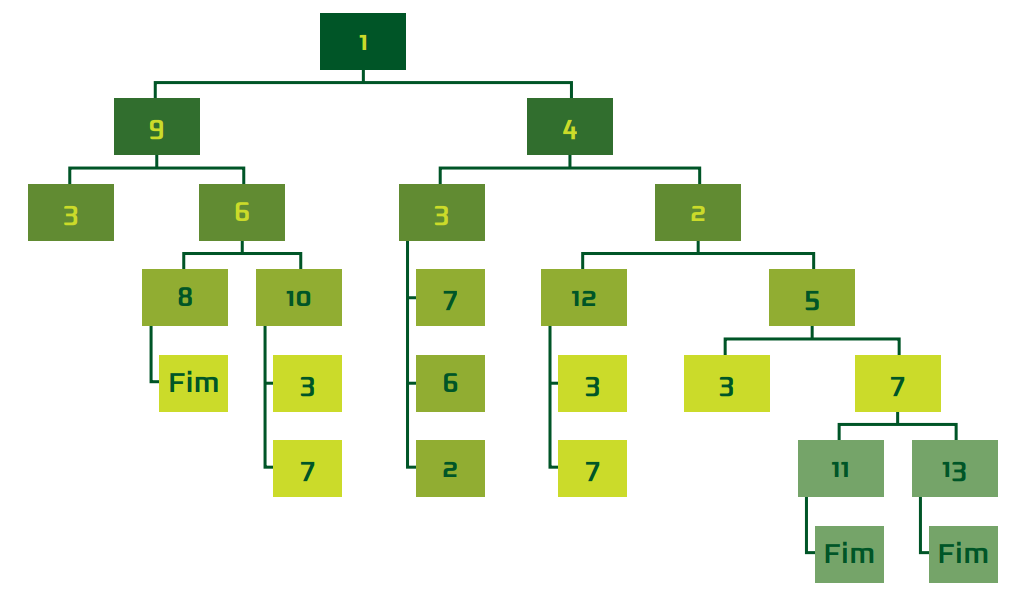
\includegraphics[scale=0.3]{Textuais/Pictures/Picture1.png}
            \fonte{\cite{Educacao_financeira_nas_escolas_professor}}\label{fig:figure-1}
        \end{figure}
        \begin{figure}
            \centering
            \caption{Momento de decisão com duas possibilidades de caminhos.}
            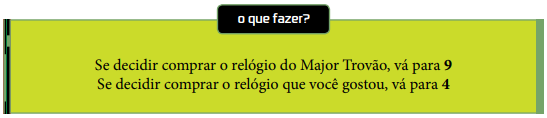
\includegraphics[scale=1]{Textuais/Pictures/Picture2.png}
            \fonte{\cite{Educacao_financeira_nas_escolas}}\label{fig:figure-2}
        \end{figure}
        \begin{figure}
            \centering
            \caption{Momento de decisão com duas possibilidades de caminhos.}
            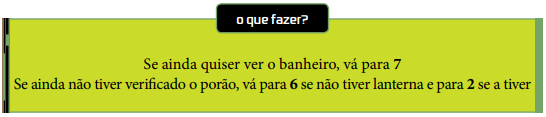
\includegraphics[scale=1]{Textuais/Pictures/Picture3.png}
            \fonte{\cite{Educacao_financeira_nas_escolas}}\label{fig:figure-3}
        \end{figure}

    \section{RPGJS}
        \textit{Framework} destinado a criação de \textit{Role-Playing Game} (RPG) na linguagem TypeScript.
        RPGJs é um projeto open source que consiste em um framework destinado à criação de Role-playing game (RPG) e
        Massively Multiplayer Online Role-Playing Game (MMORPG) que estejam disponíveis diretamente através do navegador.

        Os jogos possuem os jogadores que podem ser inseridos no mapa em diferentes coordenadas do mapa conforme a
        necessidade. Também são parte dos jogos os eventos, cenas do jogo que possibilitam ao jogador seguir pelo
        caminho escolhido durante o avanço do cenário. Além disso, é possível adicionar sons de fundo para aumentar a
        imersão no jogo. Por fim, a parte visual do jogo é realizada por meio de \textit{Tilesets} e \textit{Spritesheets}
        \cite{Documentacao_RPGJs}.

        \textit{Tileset} é uma imagem com um conjunto de \textit{Tiles} onde cada \textit{Tile} representa uma figura
        \textit{pixel art} na tela que formam um cenário, conforme figura 4. Os \textit{Tiles} podem estar ordenados de
        forma aleatória, ou seja, cada \textit{Tile} pode ter uma posição diferente em cada \textit{Tilemap}. As figuras
        no \textit{Tilemap} são baseadas na figura do jogador, assim como as cores do jogo e as cores da tela
        \cite{borges2021desenvolvimento}.

        \textit{Spritesheet}  é um conjunto de objetos 2D que descrevem os possíveis movimentos de um personagem ou
        objeto, . É uma tecnologia importante para os artistas que buscam criar imagens dinâmicas com ferramentas
        tradicionais. Ela permite baixar os custos de produção e torna possível construir imagens com qualidade, baixando ainda os
        esforços de criação. Os artistas podem alterar a aparência e o comportamento de um objeto usando ferramentas de
        desenho tradicionais, alterando ou modificando várias poses. Além disso, mesmo que essas poses intermediárias
        possam ser feitas automaticamente\cite{jones2013dynamic}.

        \begin{figure}
            \centering
            \caption{Visão da ferramenta de edição de mapas.}
            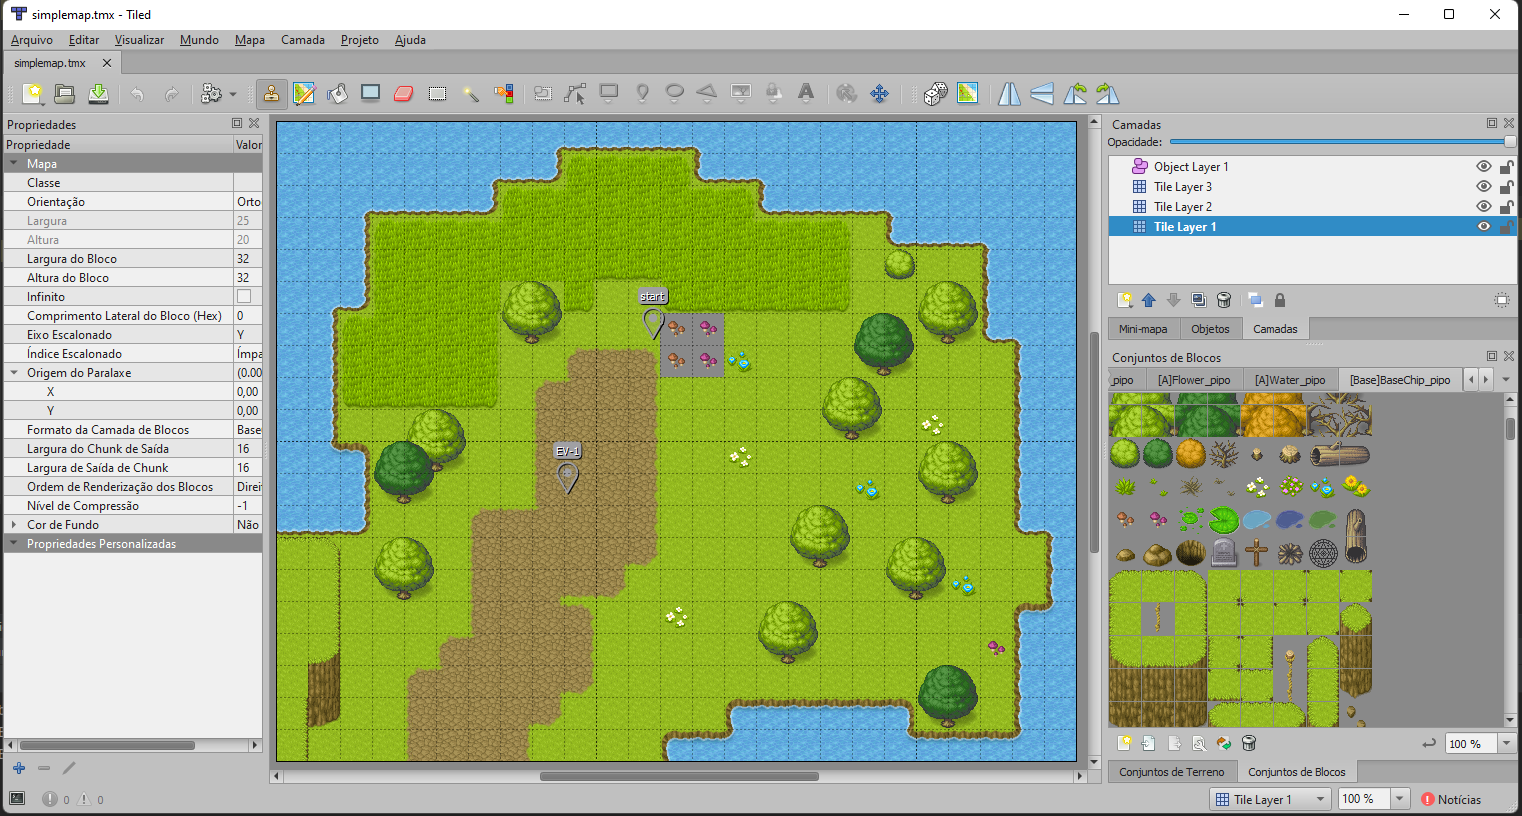
\includegraphics[scale=0.3]{Textuais/Pictures/Picture4.png}
            \fonte{\cite{Tiled}}\label{fig:figure-4}
        \end{figure}

        \begin{figure}
            \centering
            \caption{\textit{Spritesheet.}}
            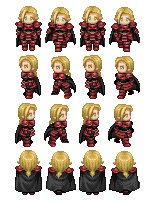
\includegraphics[scale=1.8]{Textuais/Pictures/Picture5.png}
            \fonte{\cite{Documentacao_RPGJs}}\label{fig:figure-5}
        \end{figure}


    \section{Trabalhos Correlatos}

        Nesta seção serão apresentados alguns trabalhos, que de alguma maneira se correlaciona com o presente trabalho.

        %REVER CÓPIA EXATA SBC
        \subsection{Finance Game}
            Observados os estudos, cada jogo possui uma temática diferente. O jogo Finance Game[29] busca simular a vida
            de um trabalhador em uma cidade, apresentando diferentes áreas da vida cotidiana: profissional, pessoal,
            educacional e saúde. O jogador deve administrar sua casa e sua lanchonete, através do pagamento de contas,
            compra de insumos e aplicação equilibrada  dos  seus  ganhos.  Mensagens  instrutivas  são apresentadas no
            jogo sobre situações em que o jogador precisa refletir as opções sobre promoções.

        %REVER CÓPIA EXATA SBC
        \subsection{Debt Mazer}
            No Debt Mazer[27] o jogador começa em um labirinto com vários obstáculos e armadilhas que se relacionam com
            conceitos financeiros. Existem diferentes tipos de rotas que estarão disponíveis dependendo do conhecimento
            financeiro do usuário. Chegar à casa no final do labirinto, na hora certa, é o objetivo de cada nívele, ao
            completar o labirinto, o personagem do jogador se torna o dono legal da casa.

        %REVER CÓPIA EXATA SBC
        \subsection{FinCraft}
            No FinCraft[28] para definir o conteúdo, nível e cenário, o usuário deve responder um questionário para que
            o servidor de recomendação defina um tipo de personalidade. Essa informação é armazenadaem um banco de dados
            que opera com um sistema de gerenciamento de aprendizagem e possui uma compilação dos módulos financeiros.É
            um dos estudos que apresenta em sua arquitetura o uso inteligência artificial para determinar a direção ou
            nível que o jogador deve seguir.

        %REVER CÓPIA EXATA SBC
        \subsection{DinQuiz}
            No início do jogo DinQuiz[31] o usuário recebe 50 Dins e é convidado a realizar uma das três principais
            ações: poupar, consumir e aplicar. A ação de poupar leva o jogador a uma tela de perguntas, na qual ele pode
            ser recompensado de acordo com suas respostas. Já a opção de consumir guia-o para a loja, onde o mesmo pode
            gastar seus Dins. Por fim, na opção de aplicar, ele pode escolher o tempo em que aplicao dinheiro.

        %REVER CÓPIA EXATA SBC
        \subsection{Portai\$}
            Baseado na história “O Homem mais rico da Babilônia”, no jogo Portai\$ [32] o personagem principal é
            transportado para um tempo antigo para aprender sobre finanças e libertar uma cidade da pobreza, através da
            abertura de dois portais que contém dois fantasmas: o fantasma da Hiperinflação e o fantasma do Confisco de
            Poupanças. Para abrir os portais, é necessário obter uma grande soma de dinheiro e responder 10 questões,
            que se corretas, eliminam o portal.O jogador obtémrecompensas através da profissão escolhida, e possui um
            inventário em que o jogador pode manter o dinheiro para os gastos necessários.

        \subsection{Considerações sobre os Trabalhos Correlatos}